\documentclass[11pt, a4paper]{article}
\usepackage{pdfpages}
\usepackage{parallel}
\usepackage[T2A]{fontenc}
\usepackage{ucs}
\usepackage[utf8x]{inputenc}
\usepackage[polish,english,russian]{babel}
\usepackage{hyperref}
\usepackage{rotating}
\usepackage[inner=2cm,top=1.8cm,outer=2cm,bottom=2.3cm,nohead]{geometry}
\usepackage{listings}
\usepackage{graphicx}
\usepackage{wrapfig}
\usepackage{longtable}
\usepackage{indentfirst}
\usepackage{array}
\usepackage{tikzsymbols}
\usepackage{soul}
\usepackage[ruled,vlined]{algorithm2e}
%\counterwithout{figure}{section} 

\usepackage{url}
\makeatletter
\g@addto@macro{\UrlBreaks}{\UrlOrds}
\makeatother

\newcolumntype{P}[1]{>{\raggedright\arraybackslash}p{#1}}
\frenchspacing
\usepackage{fixltx2e} %text sub- and superscripts
\usepackage{icomma} % коскі ў матэматычным рэжыме
\PreloadUnicodePage{4}

\newcommand{\longpage}{\enlargethispage{\baselineskip}}
\newcommand{\shortpage}{\enlargethispage{-\baselineskip}}

\def\switchlang#1{\expandafter\csname switchlang#1\endcsname}
\def\switchlangbe{
\let\saverefname=\refname%
\def\refname{Літаратура}%
\def\figurename{Іл.}%
}
\def\switchlangen{
\let\saverefname=\refname%
\def\refname{References}%
\def\figurename{Fig.}%
}
\def\switchlangru{
\let\saverefname=\refname%
\let\savefigurename=\figurename%
\def\refname{Литература}%
\def\figurename{Рис.}%
}

\hyphenation{admi-ni-stra-tive}
\hyphenation{ex-pe-ri-ence}
\hyphenation{fle-xi-bi-li-ty}
\hyphenation{Py-thon}
\hyphenation{ma-the-ma-ti-cal}
\hyphenation{re-ported}
\hyphenation{imp-le-menta-tions}
\hyphenation{pro-vides}
\hyphenation{en-gi-neering}
\hyphenation{com-pa-ti-bi-li-ty}
\hyphenation{im-pos-sible}
\hyphenation{desk-top}
\hyphenation{elec-tro-nic}
\hyphenation{com-pa-ny}
\hyphenation{de-ve-lop-ment}
\hyphenation{de-ve-loping}
\hyphenation{de-ve-lop}
\hyphenation{da-ta-ba-se}
\hyphenation{plat-forms}
\hyphenation{or-ga-ni-za-tion}
\hyphenation{pro-gramming}
\hyphenation{in-stru-ments}
\hyphenation{Li-nux}
\hyphenation{sour-ce}
\hyphenation{en-vi-ron-ment}
\hyphenation{Te-le-pathy}
\hyphenation{Li-nux-ov-ka}
\hyphenation{Open-BSD}
\hyphenation{Free-BSD}
\hyphenation{men-ti-on-ed}
\hyphenation{app-li-ca-tion}

\def\progref!#1!{\texttt{#1}}
\renewcommand{\arraystretch}{2} %Іначай формулы ў матрыцы зліпаюцца з лініямі
\usepackage{array}

\def\interview #1 (#2), #3, #4, #5\par{

\section[#1, #3, #4]{#1 -- #3, #4}
\def\qname{LVEE}
\def\aname{#1}
\def\q ##1\par{{\noindent \bf \qname: ##1 }\par}
\def\a{{\noindent \bf \aname: } \def\qname{L}\def\aname{#2}}
}

\def\interview* #1 (#2), #3, #4, #5\par{

\section*{#1\\{\small\rm #3, #4. #5}}
\ifx\ParallelWhichBox\undefined%
    \addcontentsline{toc}{section}{#1, #3, #4}%
\else%
\ifnum\ParallelWhichBox=0%
    \addcontentsline{toc}{section}{#1, #3, #4}%
\fi\fi%

\def\qname{LVEE}
\def\aname{#1}
\def\q ##1\par{{\noindent \bf \qname: ##1 }\par}
\def\a{{\noindent \bf \aname: } \def\qname{L}\def\aname{#2}}
}

\newcommand{\interviewfooter}[1]{
\vskip 1em
\noindent \textit{#1}
}


\begin{document}

\title{1994 "--- Memorex trackball}
\date{}
\maketitle

Трекбол Memorex, показанный на рис. \ref{fig:MemorexPic}, выпускался калифорнийской компанией Memtek Products inc. При этом фактическое производство типичным для середины 90-х годов образом велось на Тайвани.

\begin{figure}[h]
    \centering
    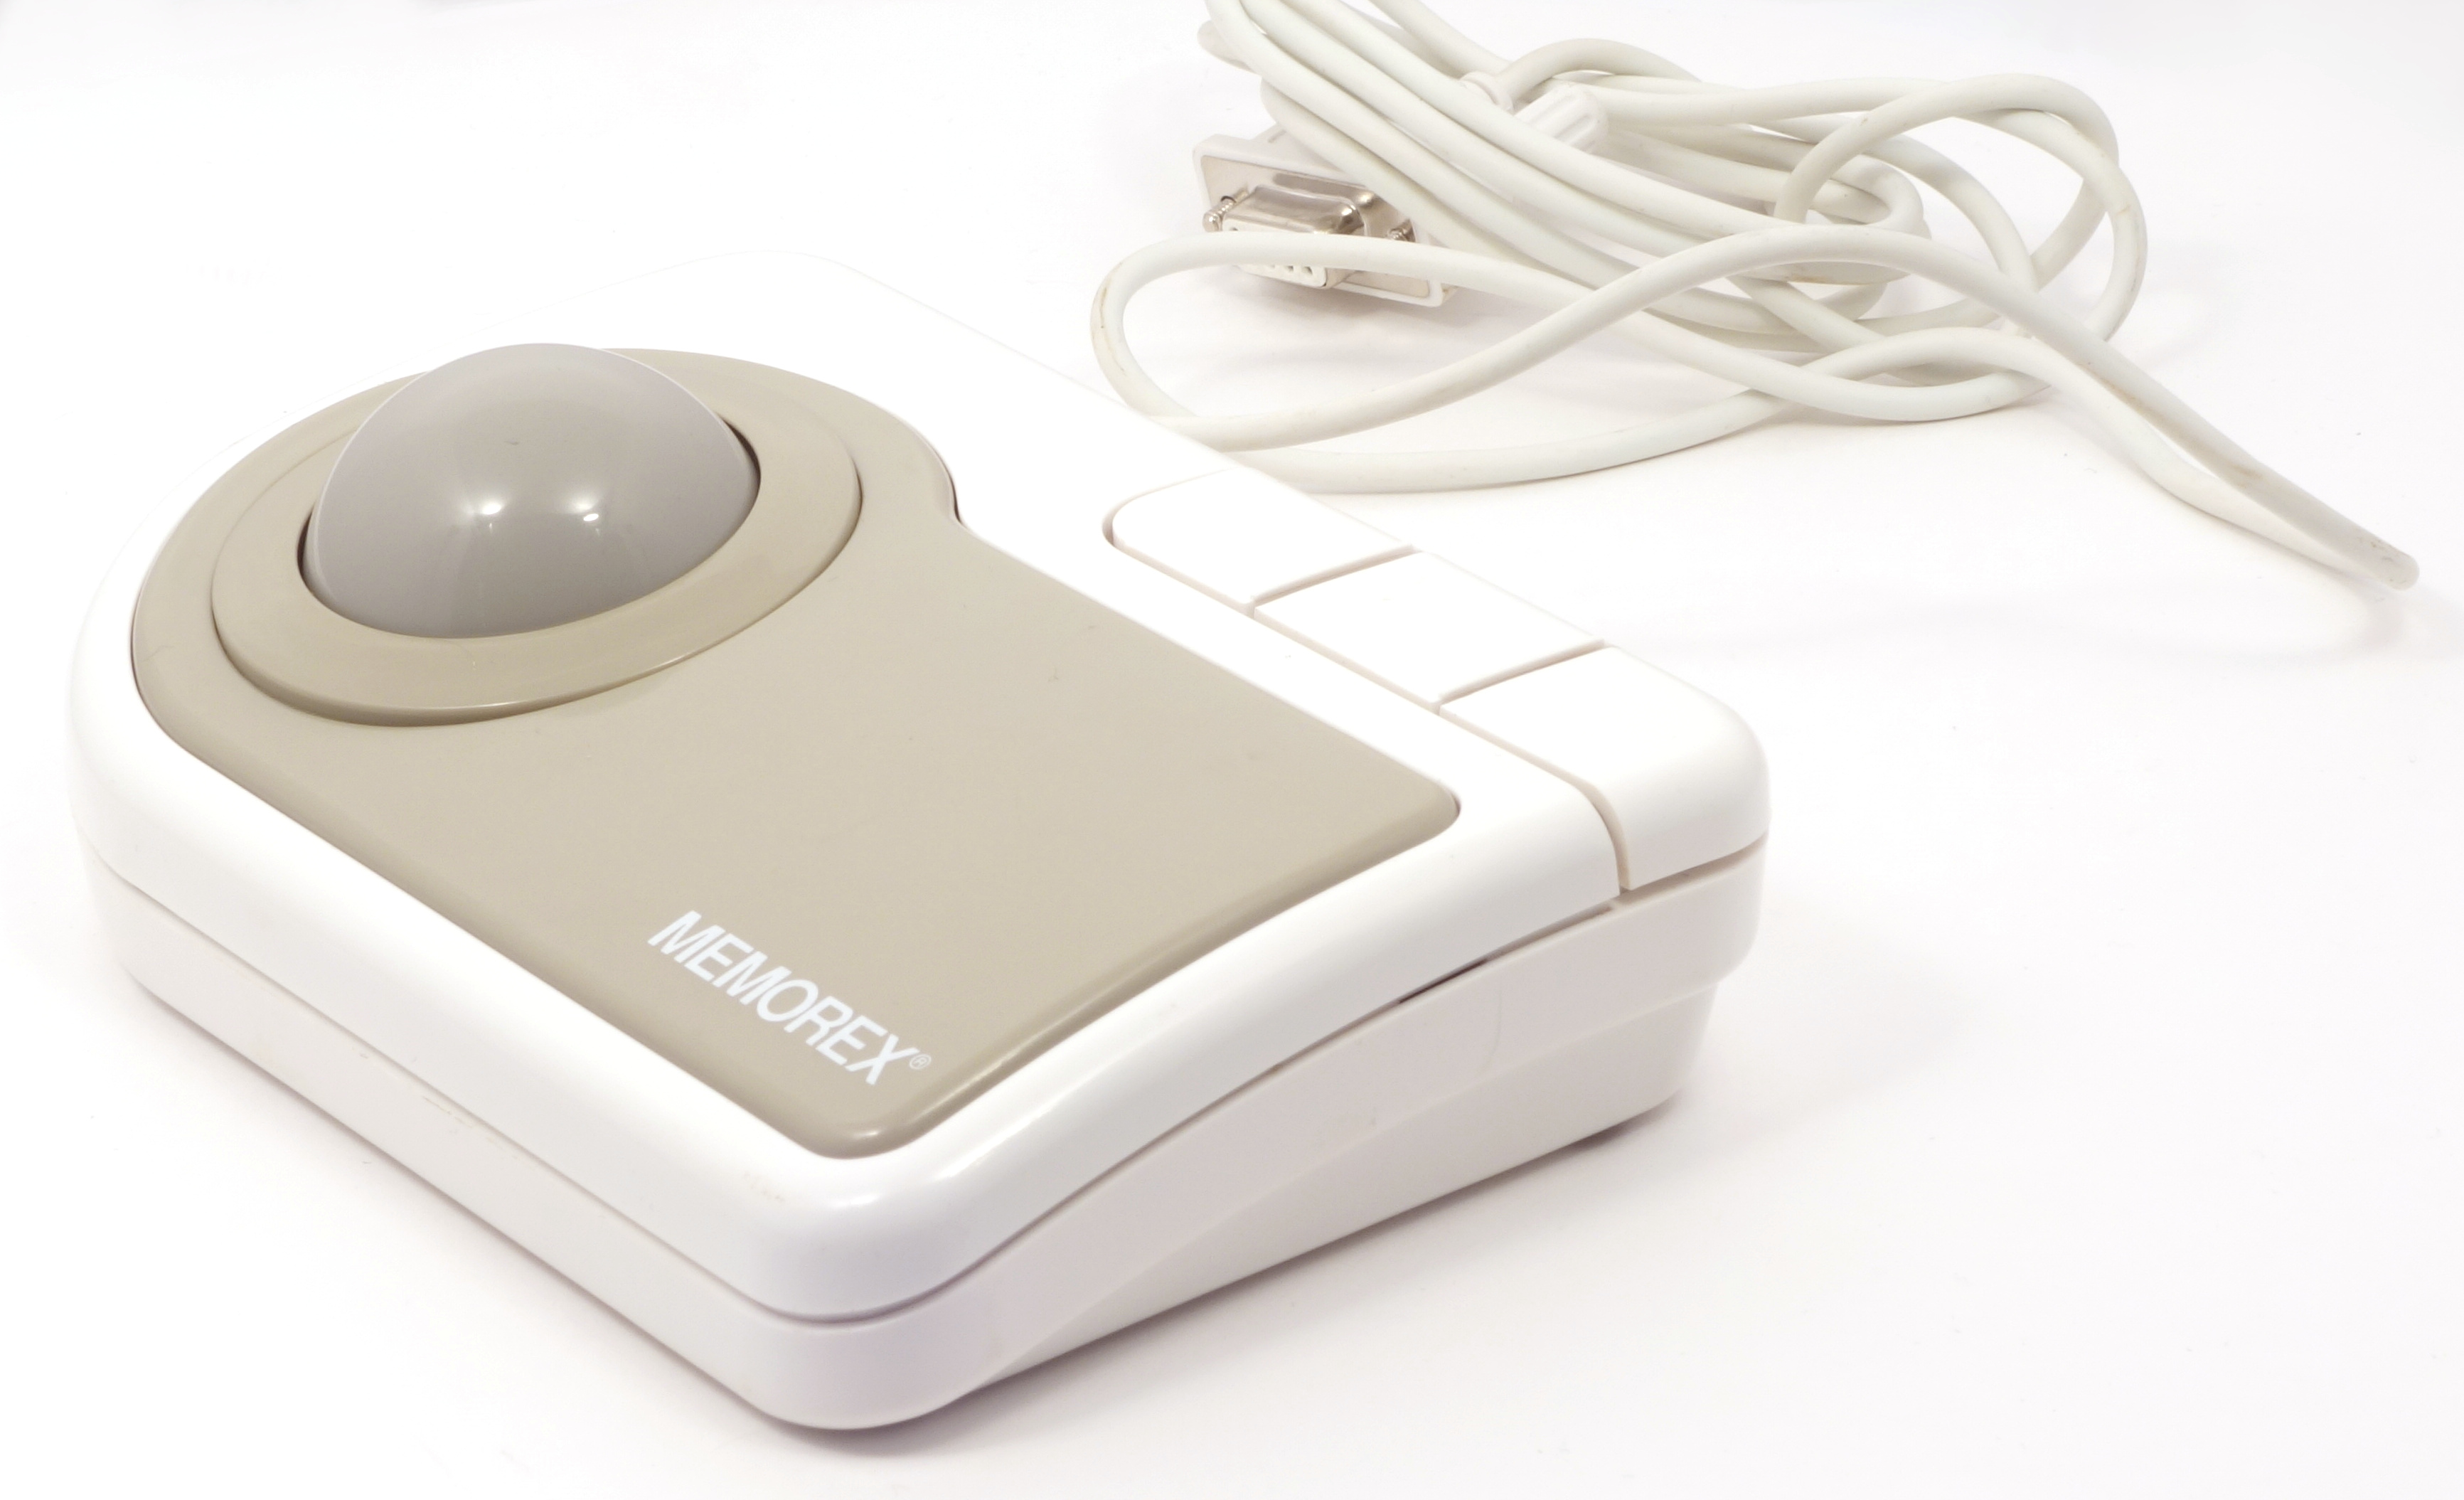
\includegraphics[scale=0.5]{1994_memorex_trackball/pic_30.jpg}
    \caption{Вид трекбола Memorex}
    \label{fig:MemorexPic}
\end{figure}

Корпус трекбола является асимметричным, выполнен в минималистичном стиле из глянцево-белого пластика с коричневой вставкой.

\begin{figure}[h]
    \centering
    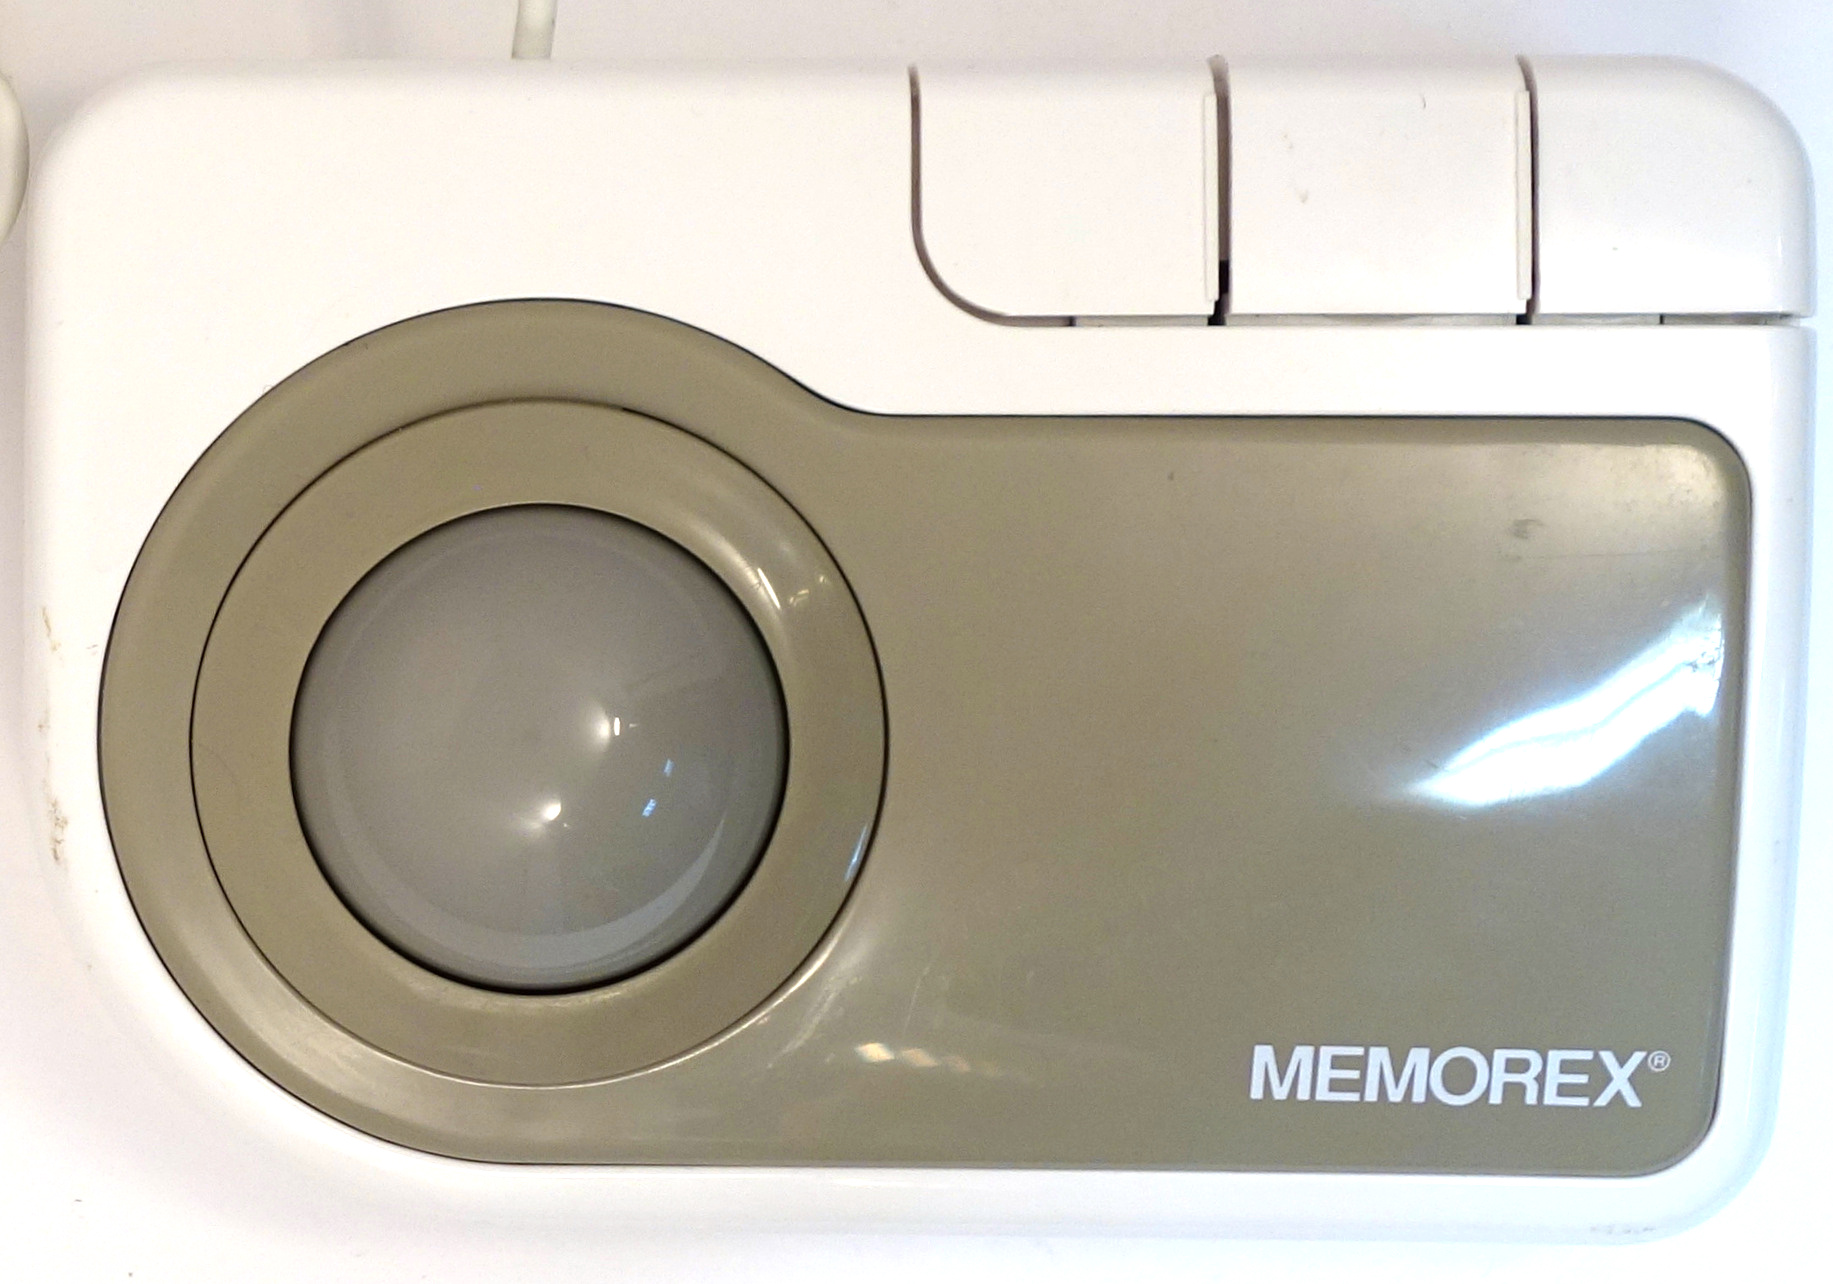
\includegraphics[scale=0.45]{1994_memorex_trackball/top_30.jpg}
    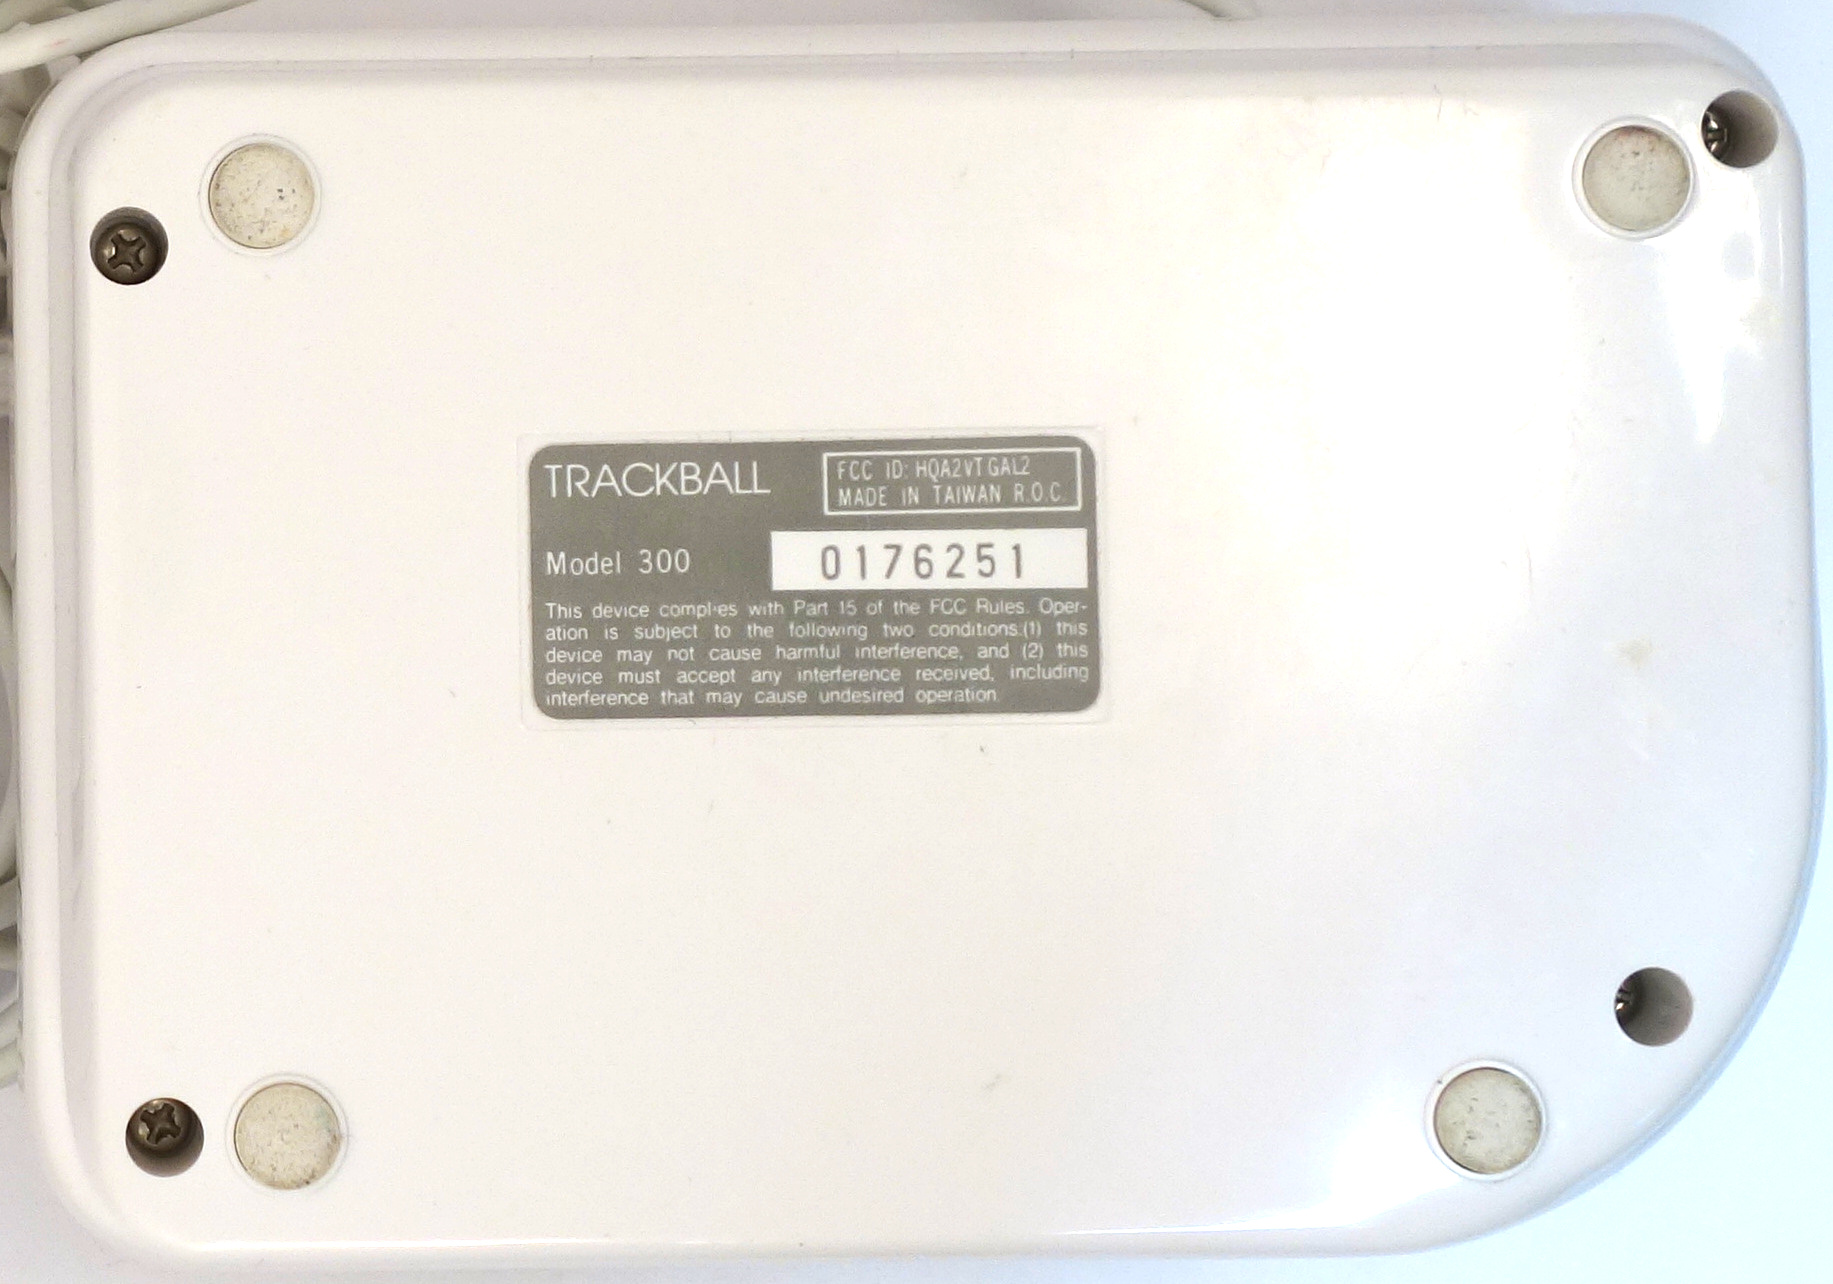
\includegraphics[scale=0.45]{1994_memorex_trackball/bottom_30.jpg}
    \caption{Easy Options, вид сверху и снизу}
    \label{fig:MemorexTopBottom}
\end{figure}

Как можно видеть на рис. \ref{fig:MemorexSize}, этот манипулятор имеет сравнительно небольшие размеры.
На упаковке трекбола и в руководстве пользователя использован подзаголовок "Stationary Mouse", очевидно позаимствованный у выпущенной годом ранее модели трекбола Logitech TrackMan Stationary Mouse, и подчеркивается удобство его использования в условиях ограниченного рабочего пространства.

\begin{figure}[h]
    \centering
    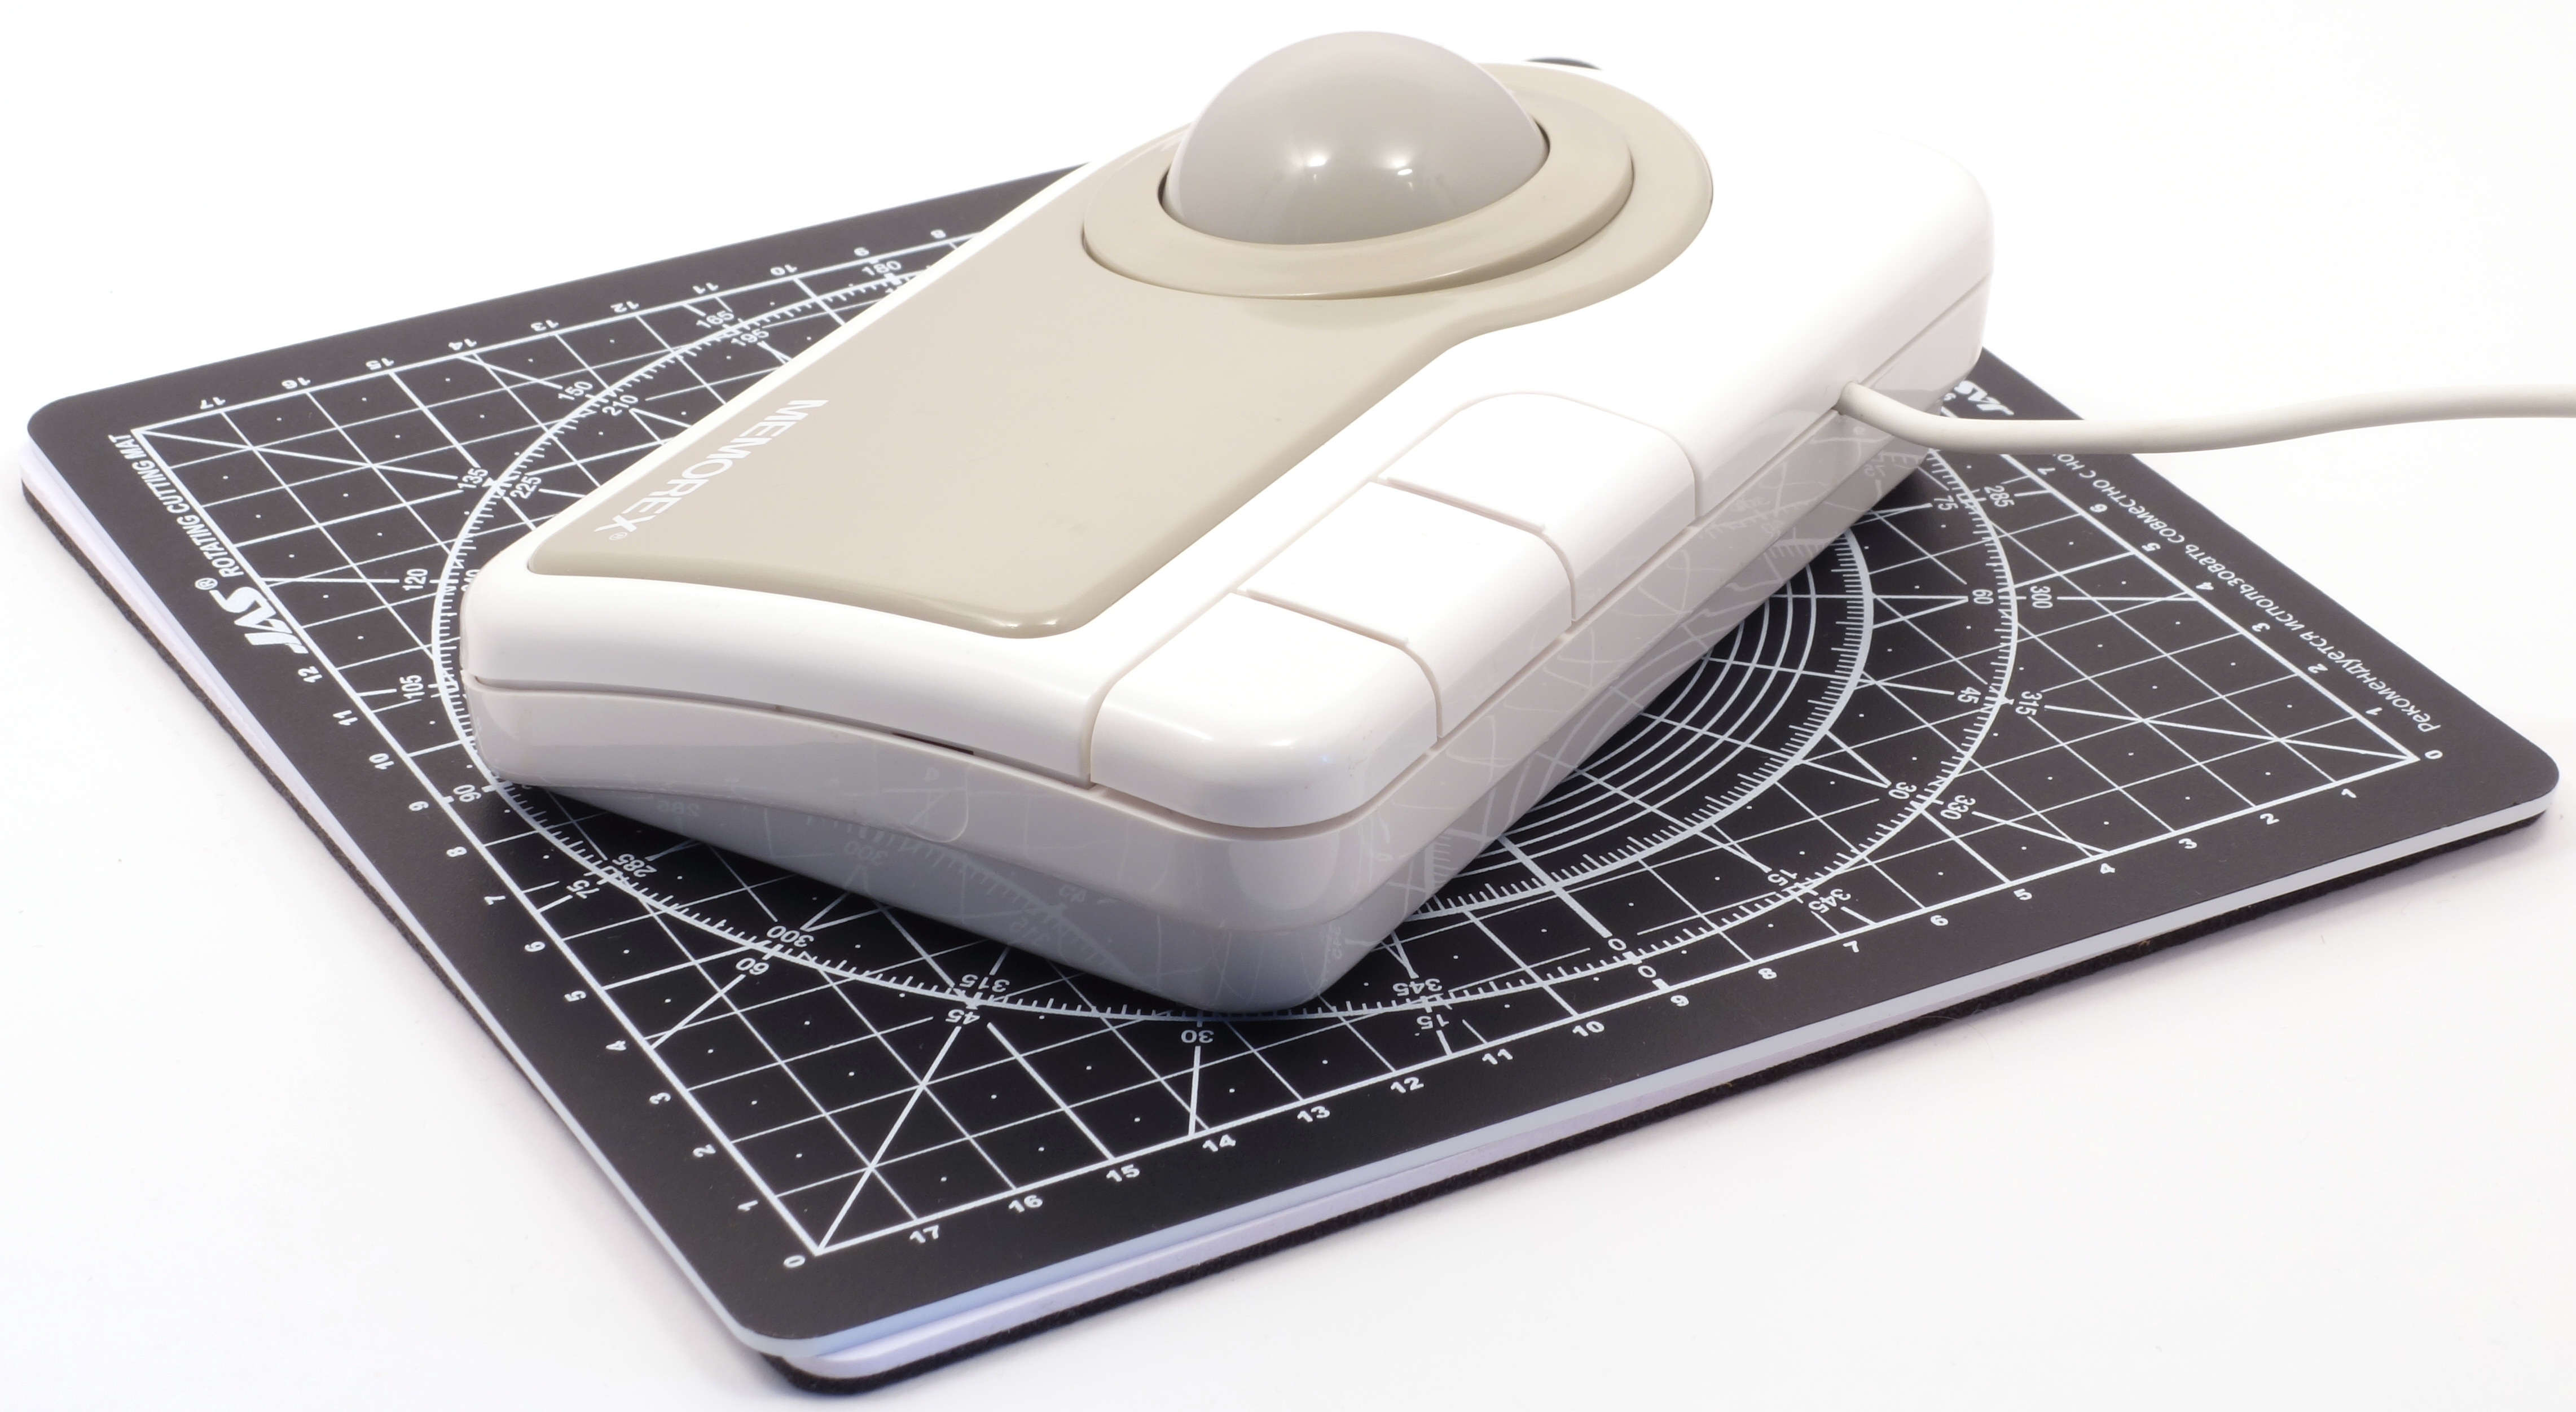
\includegraphics[scale=0.35]{1994_memorex_trackball/size_30.jpg}
    \caption{Трекбол Memorex на размерном коврике с шагом сетки 1 см}
    \label{fig:MemorexSize}
\end{figure}

Трекбол рассчитан на управление правой рукой, а его форма в значительной степени инспирирована другим продуктом Logitech - LOGiTECH, в который также рассчитан на горизонтальное расположение кисти руки и вращение шара большим пальцем (рис. \ref{fig:MemorexHand}). По замыслу Logitech, данная форма является лучше соответствует анатомическому строению кисти (в рекламе форма классических симметричных трекболов противопоставлялась подобной форме как <<устройство для инопланетян>> \cite{adv}).

\begin{figure}[h]
    \centering
    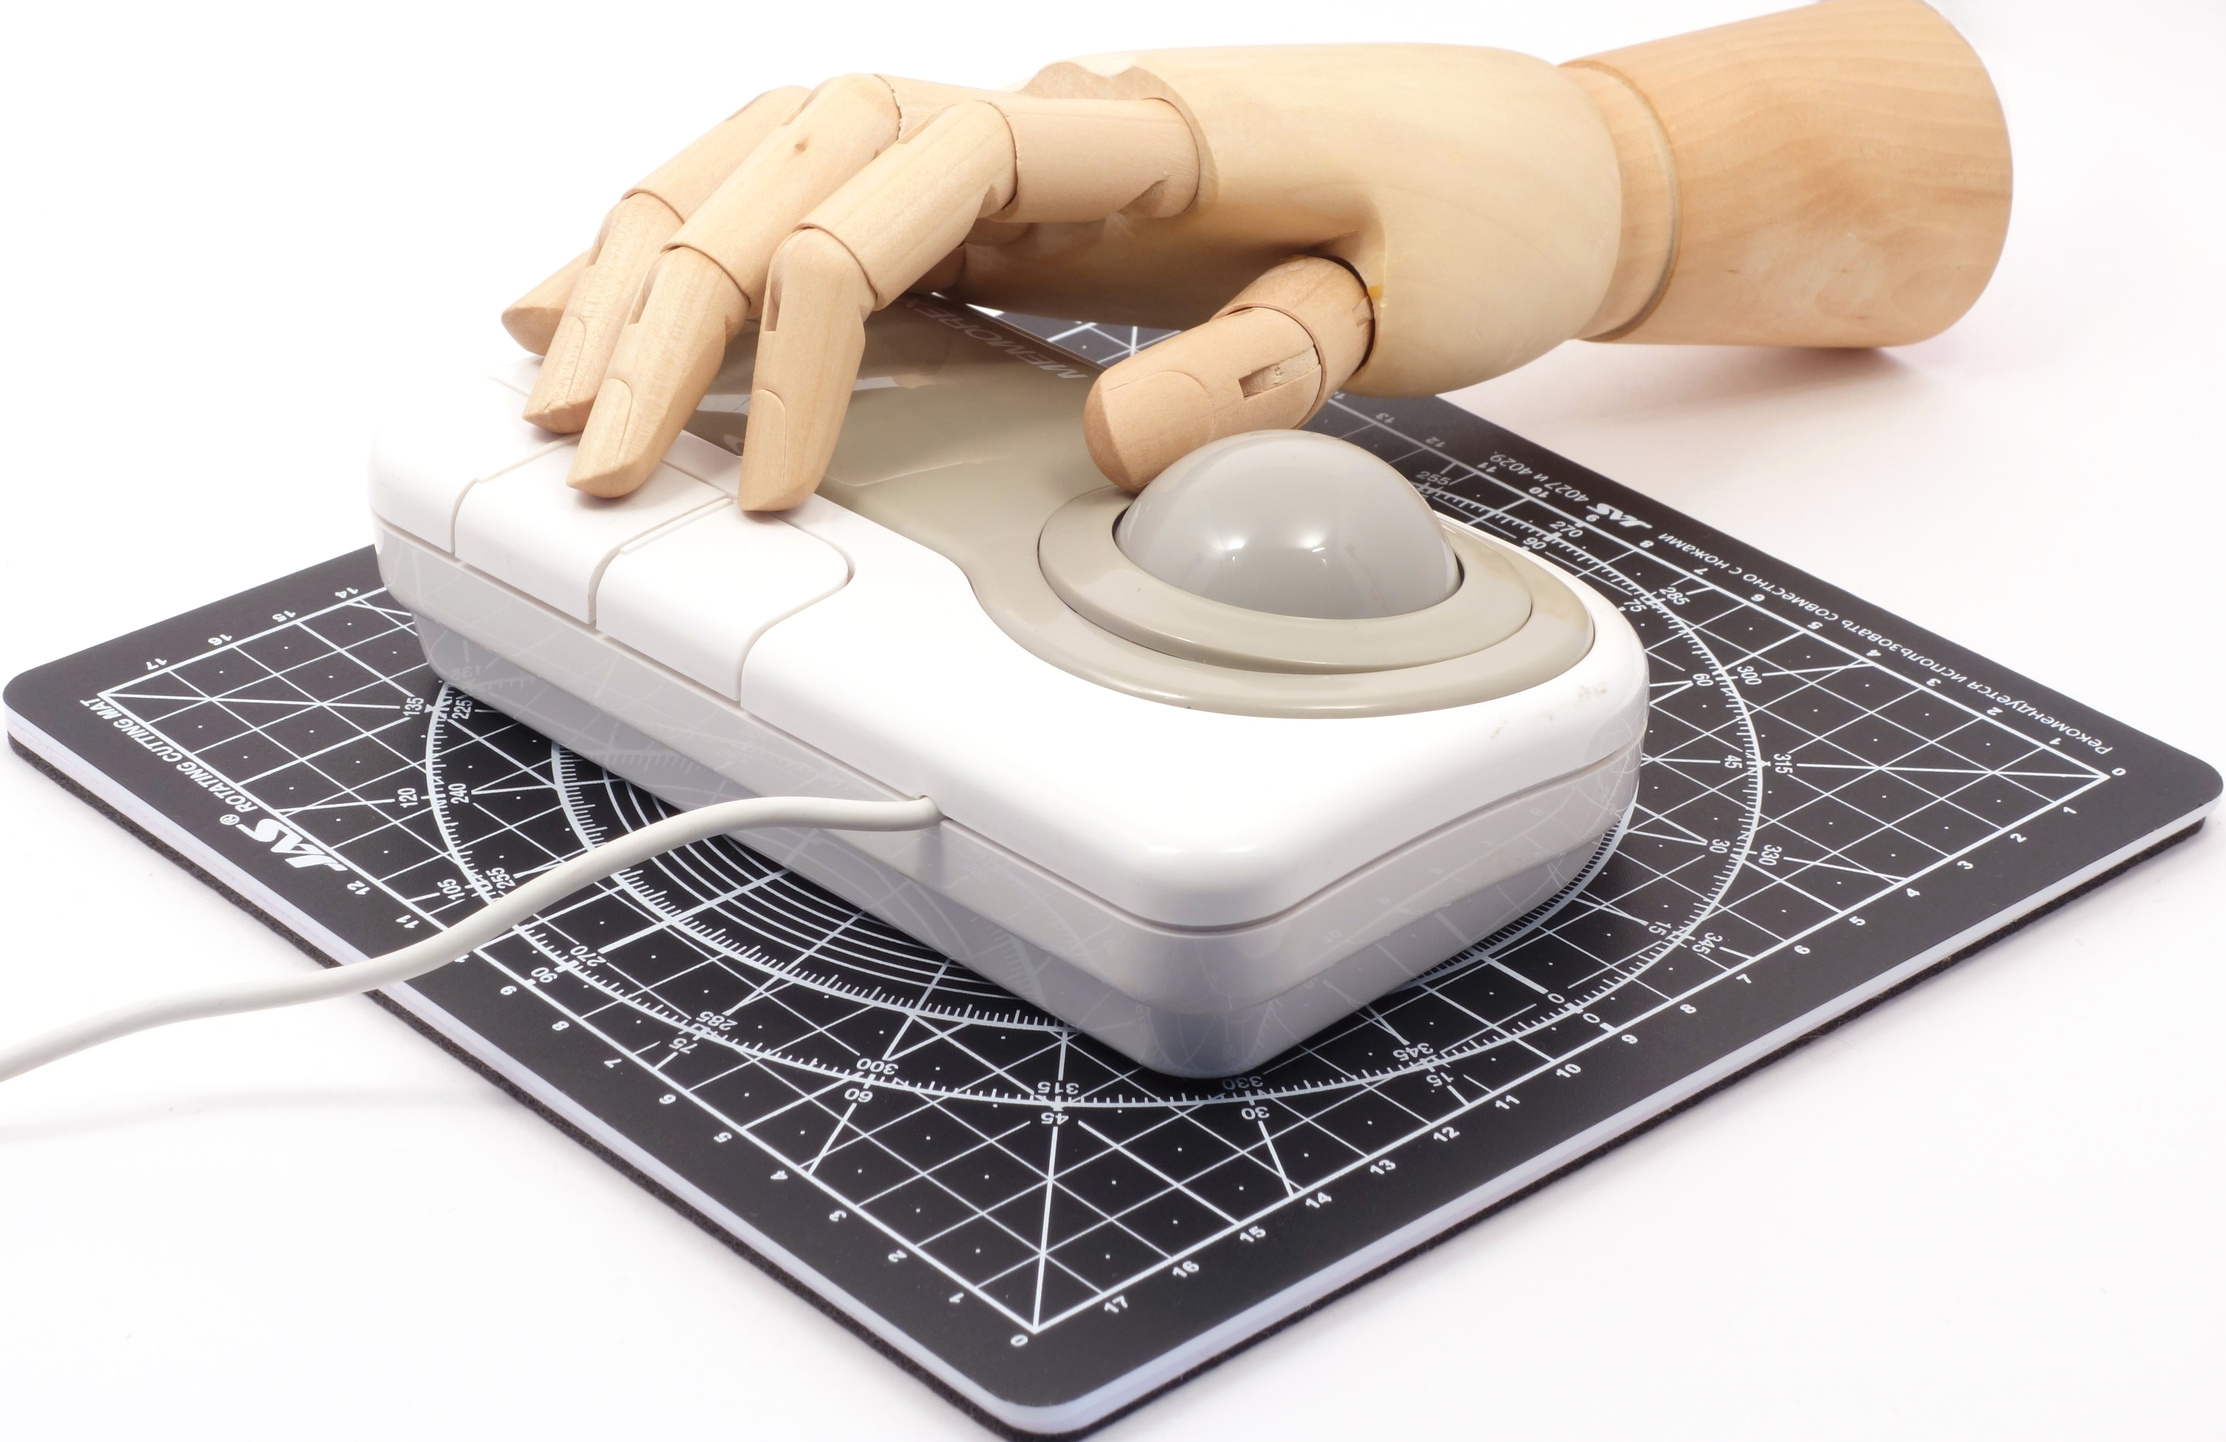
\includegraphics[scale=0.2]{1994_memorex_trackball/hand_30.jpg}
    \caption{Трекбол Memorex в комплекте с моделью руки человека}
    \label{fig:MemorexHand}
\end{figure}

Внутреннее устройство трекбола показано на рис. \ref{fig:MemorexInside}, что позволяет классифицировать его как типичное оптомеханическое устройство середины 90-х годов, как в плане реализации энкодера, так и в плане компоновки, оставлявшей значительный объем пустого пространства внутри корпуса.

\begin{figure}[h]
    \centering
    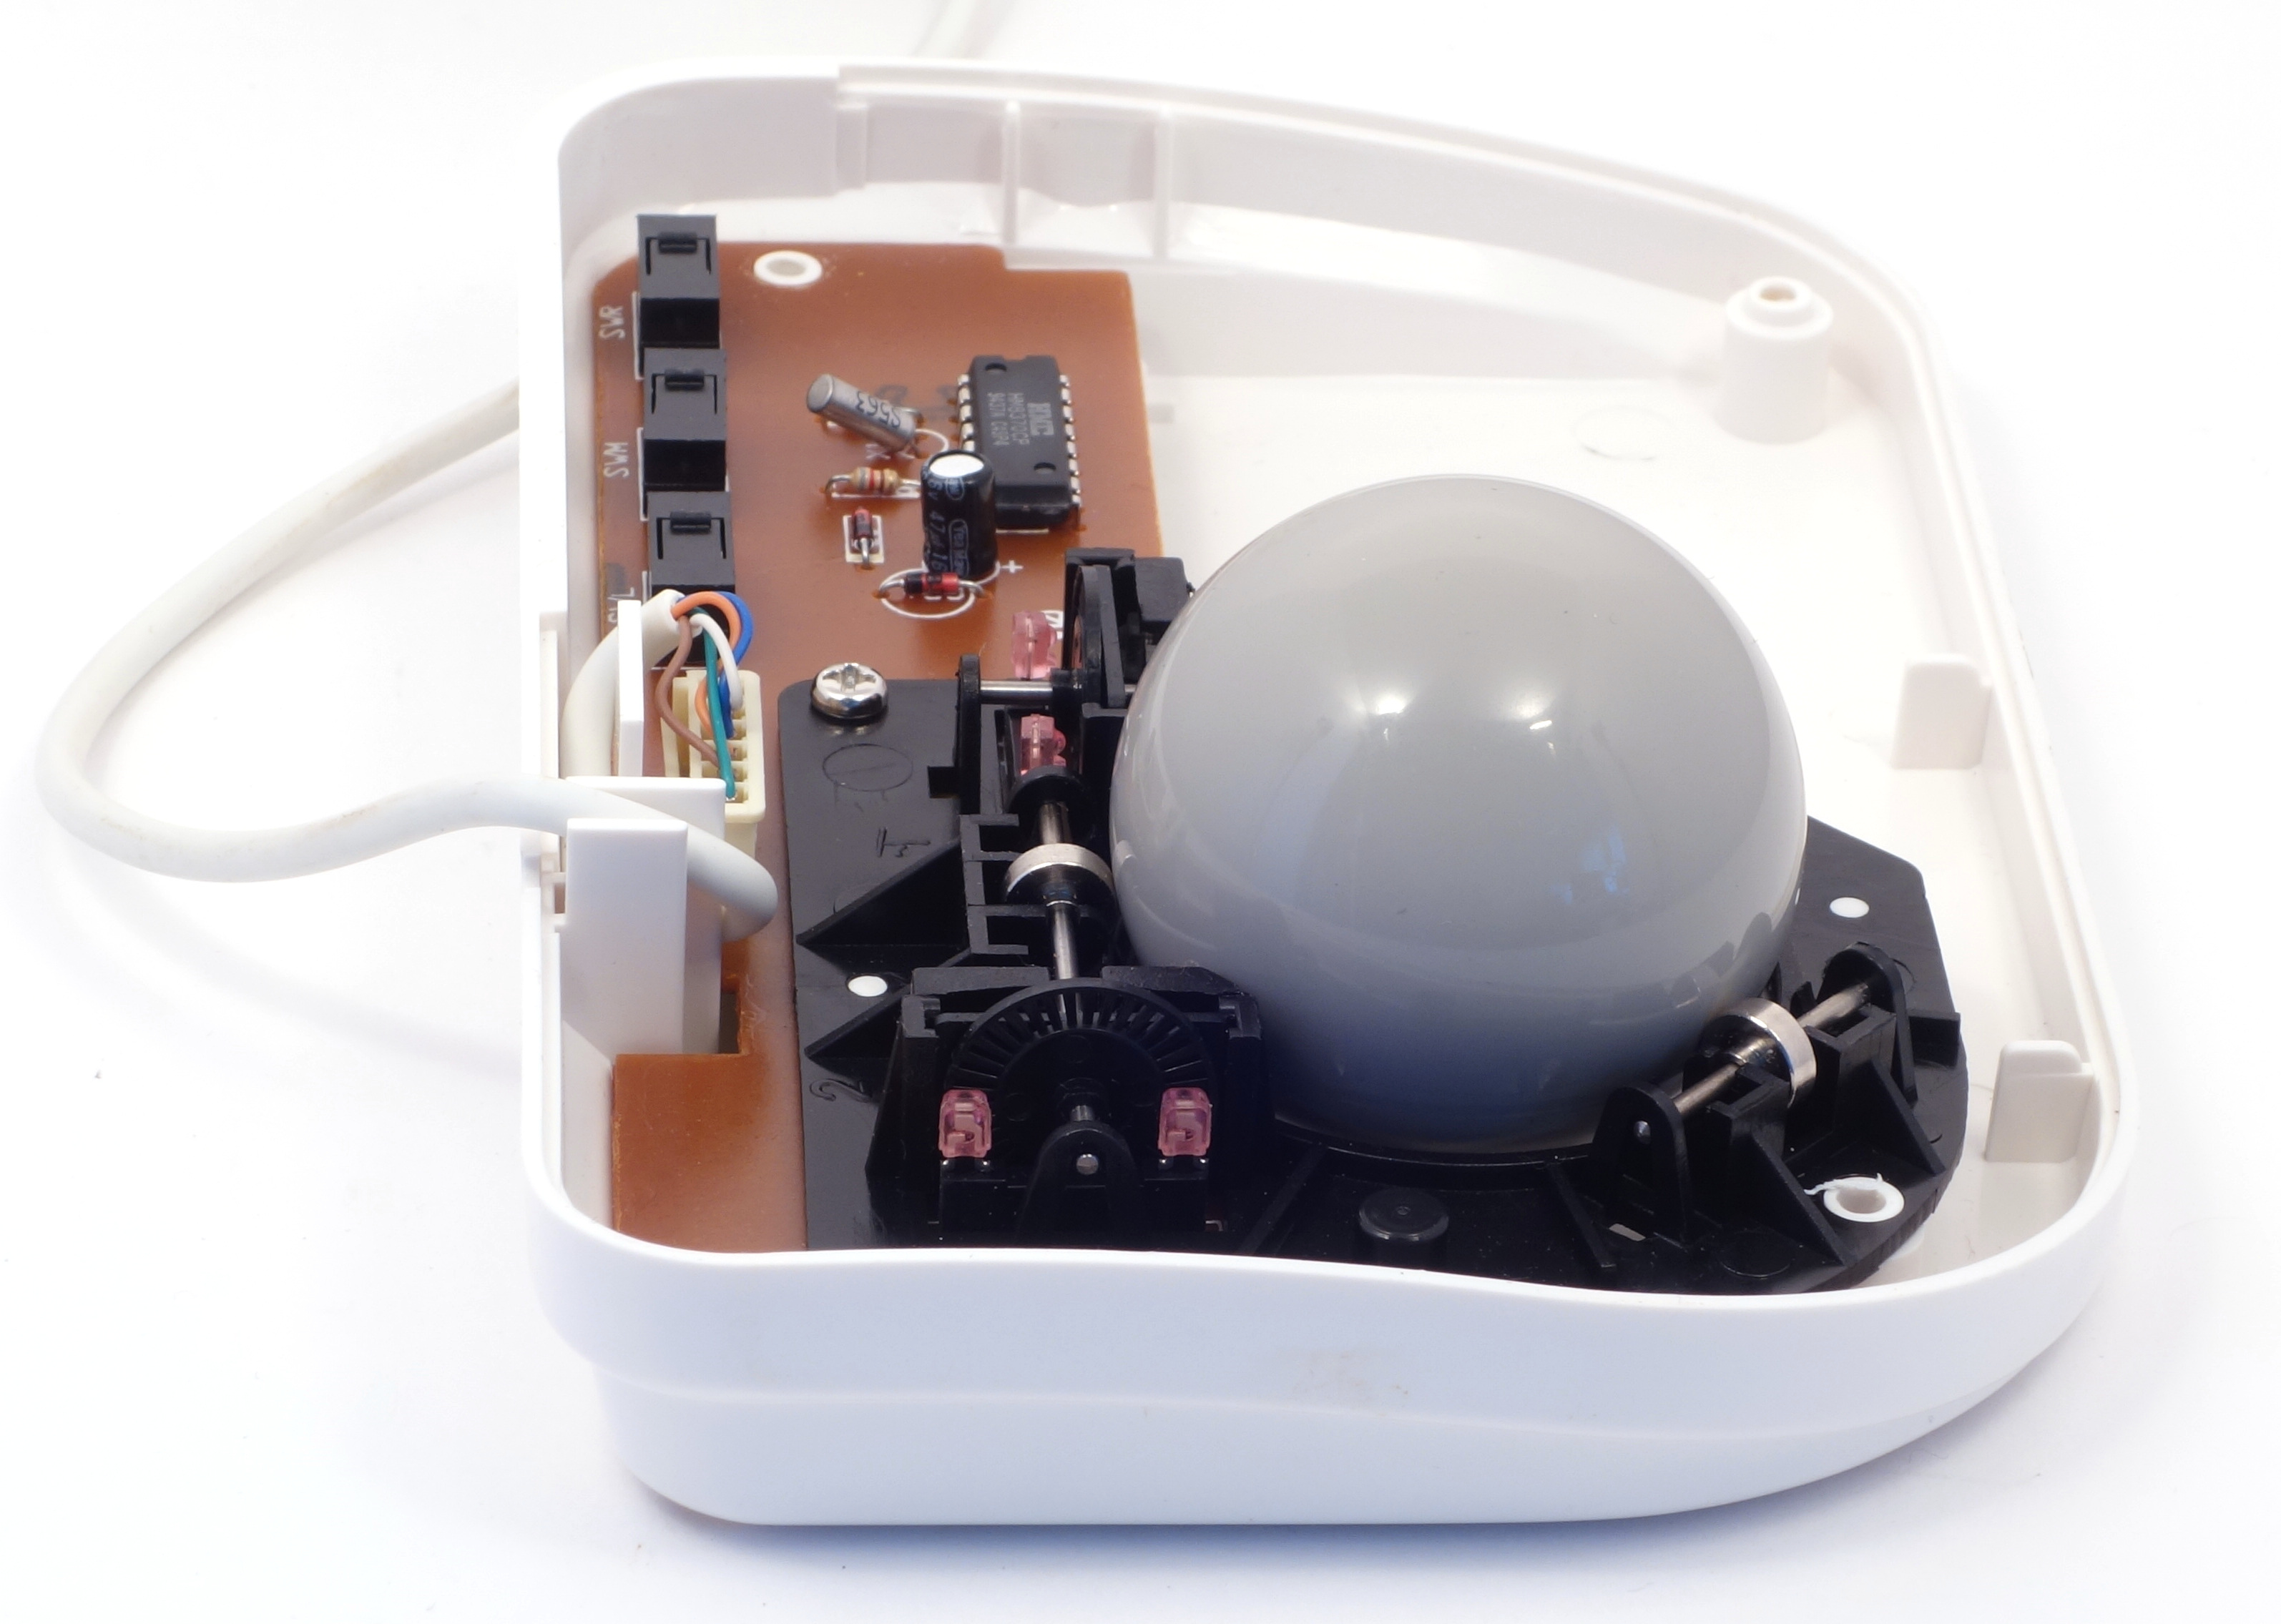
\includegraphics[scale=0.6]{1994_memorex_trackball/inside_30.jpg}
    \caption{Memorex в разобранном виде}
    \label{fig:MemorexInside}
\end{figure}

\begin{thebibliography}{9}
\bibitem {adv} Not every kind of pointing device fits your kind of hand (LOGiTECH TrackMan tadvertising). // PC Magazine. V.~8, No.~19. November, 1989, pp. 360-361. \url{https://archive.org/details/PC-Mag-1989-11-14/page/n361}
\end{thebibliography}
\end{document}
